\section{SCD}
\thispagestyle{fancy}


``System Control Diagram'' (\gls{SCD})  er eit grafisk dokumentasjonsverktøy beskrevet i \gls{IEC} \gls{PAS} 63131.\newline
 \gls{SCD} blir brukt for å vise relasjonane mellom prosessens komponentar og programmet som styrer dei og skiljer seg frå ein \gls{PID}
 som dokumenterer alt fysisk utstyr.

 Vi ynskjer å bruke \gls{SCD} som eit planleggingsverktøy for programstrukteren. \gls{SCD} inneheld \gls{IEC} funksjonsblokk maler noko som gjer at ein kan
 planlegge programmering av anlegget før ein har skreve sjølve \gls{IEC} blokk koden.
 Diagrammet gir oss mulighet til å visualsere, teikne og kople \gls{IEC} blokkene mot komponentane på anlegget og 
 gir oss også ein unik moglegheit for å kunne dokumentere arbeidet og vil gi ein grafisk representasjon
 av styringsform og løysningar som blir valgt.

 Vi har kontakta MIDTechology \citep{MIDT} som er som er eit selskap som utviklar programvare for \gls{SCD} og vi har fått utlevert studentlisensar
 til programvaren. Vi vil bruke dette programmet for planlegging og dokumentering av koden til reiseanlegget på Sande.

 \begin{figure}[htbp]
    \centering
    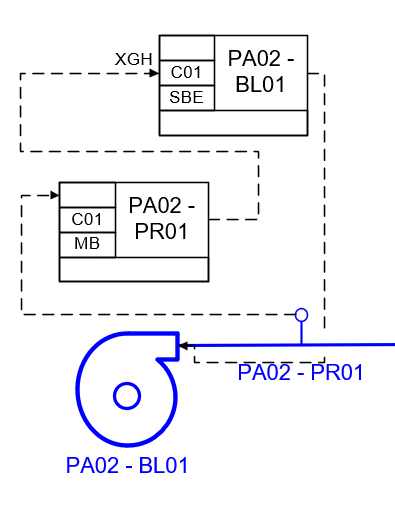
\includegraphics[width=0.35\textwidth]{Bilder/Visio_eksempel.png}
    \caption{Eksempel av \gls{SCD}}\label{fig:SCD eksempel}    
\end{figure}

\newpage